\documentclass{article}
\usepackage{tikz}
\usetikzlibrary{shapes.geometric, arrows.meta, positioning, calc, fit}

\begin{document}
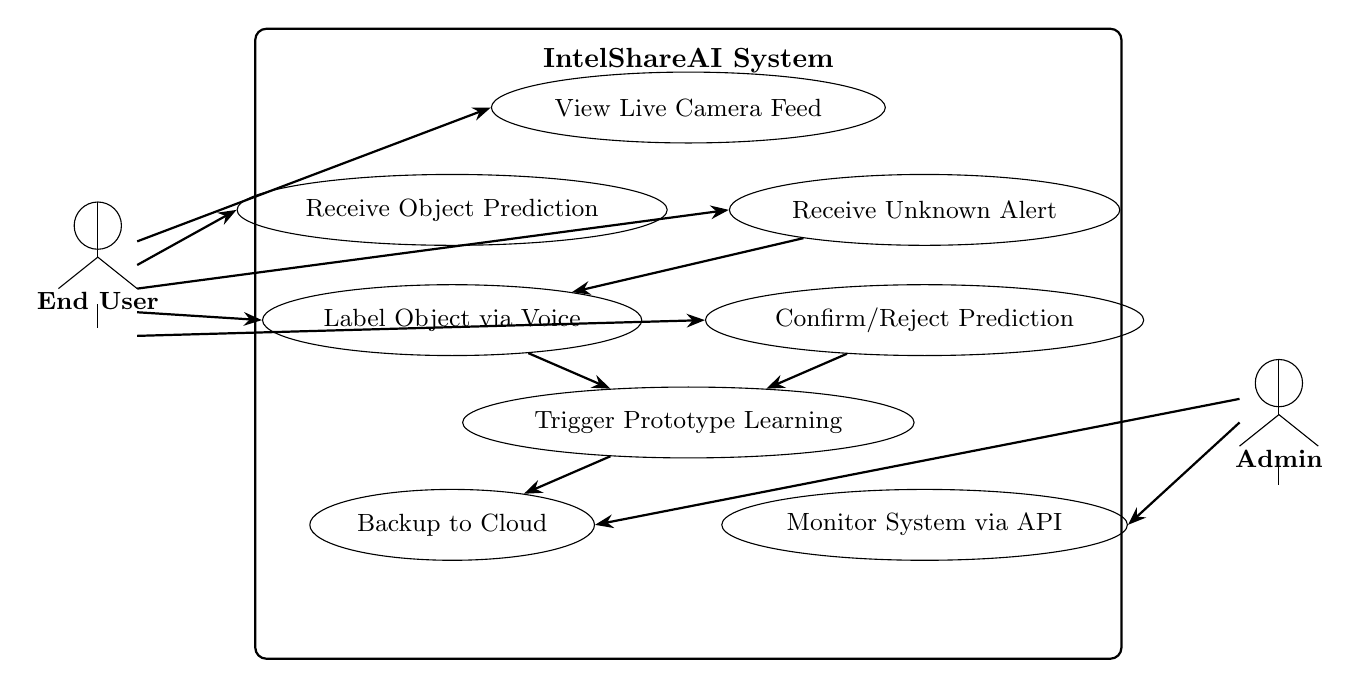
\begin{tikzpicture}[
    actor/.style={},
    usecase/.style={ellipse, minimum width=2.8cm, minimum height=0.9cm, text centered, draw=black, font=\small, inner sep=2pt},
    arrow/.style={thick, -Stealth}
]
    % System boundary
    \draw [thick, rounded corners] (-5.5, -6.5) rectangle (5.5, 1.5);
    \node [font=\bfseries] at (0, 1.1) {IntelShareAI System};

    % Use cases
    \node (uc1) [usecase] at (0, 0.5) {View Live Camera Feed};
    \node (uc2) [usecase] at (-3, -0.8) {Receive Object Prediction};
    \node (uc3) [usecase] at (3, -0.8) {Receive Unknown Alert};
    \node (uc4) [usecase] at (-3, -2.2) {Label Object via Voice};
    \node (uc5) [usecase] at (3, -2.2) {Confirm/Reject Prediction};
    \node (uc6) [usecase] at (0, -3.5) {Trigger Prototype Learning};
    \node (uc7) [usecase] at (-3, -4.8) {Backup to Cloud};
    \node (uc8) [usecase] at (3, -4.8) {Monitor System via API};

    % Actors
    \node (user) [actor] at (-7.5, -1.5) {};
    \node [below=0.1cm of user, font=\small\bfseries] {End User};
    \draw (-7.5, -1) circle (0.3);
    \draw (-7.5, -0.7) -- (-7.5, -1.4);
    \draw (-7.5, -2.0) -- (-7.5, -2.3);
    \draw (-7.5, -1.4) -- (-8.0, -1.8);
    \draw (-7.5, -1.4) -- (-7.0, -1.8);

    \node (admin) [actor] at (7.5, -3.5) {};
    \node [below=0.1cm of admin, font=\small\bfseries] {Admin};
    \draw (7.5, -3) circle (0.3);
    \draw (7.5, -2.7) -- (7.5, -3.4);
    \draw (7.5, -4.0) -- (7.5, -4.3);
    \draw (7.5, -3.4) -- (7.0, -3.8);
    \draw (7.5, -3.4) -- (8.0, -3.8);

    % Connections - User
    \draw [arrow] (-7, -1.2) -- (uc1.west);
    \draw [arrow] (-7, -1.5) -- (uc2.west);
    \draw [arrow] (-7, -1.8) -- (uc3.west);
    \draw [arrow] (-7, -2.1) -- (uc4.west);
    \draw [arrow] (-7, -2.4) -- (uc5.west);

    % Connections - Admin
    \draw [arrow] (7, -3.2) -- (uc7.east);
    \draw [arrow] (7, -3.5) -- (uc8.east);

    % Internal connections
    \draw [arrow] (uc3) -- (uc4);
    \draw [arrow] (uc4) -- (uc6);
    \draw [arrow] (uc5) -- (uc6);
    \draw [arrow] (uc6) -- (uc7);
\end{tikzpicture}
\end{document}
